\documentclass[a4paper, 10pt, ]{article}

\usepackage[slovak]{babel}





\usepackage[utf8]{inputenc}
\usepackage[T1]{fontenc}

\usepackage[left=4cm,
			right=4cm,
            % left=2.5cm,
			% right=5.5cm,
			top=2.1cm,
			bottom=2.6cm,
			footskip=7.5mm,
			% twoside,
			marginparwidth=3.0cm,
			%showframe,
			]{geometry}

\usepackage{graphicx}
\usepackage[dvipsnames]{xcolor}
% https://en.wikibooks.org/wiki/LaTeX/Colors


% ------------------------------

\usepackage{lmodern}

\usepackage[tt={oldstyle=false,proportional=true,monowidth}]{cfr-lm}

% ------------------------------

\usepackage{amsmath}
\usepackage{amssymb}
\usepackage{amsthm}

\usepackage{booktabs}
\usepackage{multirow}
\usepackage{array}
\usepackage{dcolumn}


\usepackage[singlelinecheck=true]{subfig}


% ------------------------------


\def\naT{\mathsf{T}}

\hyphenpenalty=6000
\tolerance=1000




% ------------------------------


\makeatletter

	\def\@seccntformat#1{\protect\makebox[0pt][r]{\csname the#1\endcsname\hspace{4mm}}}

	\def\cleardoublepage{\clearpage\if@twoside \ifodd\c@page\else
	\hbox{}
	\vspace*{\fill}
	\begin{center}
	\phantom{}
	\end{center}
	\vspace{\fill}
	\thispagestyle{empty}
	\newpage
	\if@twocolumn\hbox{}\newpage\fi\fi\fi}

	\newcommand\figcaption{\def\@captype{figure}\caption}
	\newcommand\tabcaption{\def\@captype{table}\caption}

\makeatother


% ------------------------------




\usepackage{fancyhdr}
\fancypagestyle{plain}{%
\fancyhf{} % clear all header and footer fields
\fancyfoot[C]{\sffamily {\bfseries \thepage}\ | {\scriptsize\oznacenieCasti}}
\renewcommand{\headrulewidth}{0pt}
\renewcommand{\footrulewidth}{0pt}}
\pagestyle{plain}


% ------------------------------


\usepackage{titlesec}
\titleformat{\paragraph}[hang]{\sffamily  \bfseries}{}{0pt}{}
\titlespacing*{\paragraph}{0mm}{3mm}{1mm}
\titlespacing*{\subparagraph}{0mm}{3mm}{1mm}

\titleformat*{\section}{\sffamily\Large\bfseries}
\titleformat*{\subsection}{\sffamily\large\bfseries}
\titleformat*{\subsubsection}{\sffamily\normalsize\bfseries}






% ------------------------------

\PassOptionsToPackage{hyphens}{url}
\usepackage[pdfauthor={},
			pdftitle={},
			pdfsubject={},
			pdfkeywords={},
			% hidelinks,
			colorlinks=false,
			breaklinks,
			]{hyperref}


% ------------------------------


\graphicspath{%
{../fig_standalone/}%
{../../PY/fig/}%
{../../PY/jupynotex/fig/}%
{../../ML/fig/}%
{./fig/}%
}



% ------------------------------

\usepackage{enumitem}

\usepackage{lettrine}

% ------------------------------


\usepackage{microtype}


% ------------------------------

\usepackage[titles]{tocloft}

\setlength{\cftsecindent}{-12mm}
\setlength{\cftsecnumwidth}{12mm}
\renewcommand{\cftsecpresnum}{\hfill}
\renewcommand{\cftsecaftersnum}{\hspace{4mm}}

\setlength{\cftsubsecindent}{-12mm}
\setlength{\cftsubsecnumwidth}{16mm} % 12 + 4
\renewcommand{\cftsubsecpresnum}{\hfill}
\renewcommand{\cftsubsecaftersnum}{\hspace{8mm}} % 4 + 4 mm

\setlength{\cftsubsubsecindent}{-12mm}
\setlength{\cftsubsubsecnumwidth}{20mm} % 12 + 4 + 4
\renewcommand{\cftsubsubsecpresnum}{\hfill}
\renewcommand{\cftsubsubsecaftersnum}{\hspace{12mm}} % 4 + 4 + 4 mm

\renewcommand{\cftsecpagefont}{\lstyle \bfseries}
\renewcommand{\cftsubsecpagefont}{\lstyle}
\renewcommand{\cftsubsubsecpagefont}{\lstyle}



\setlength{\cftparaindent}{-16mm}
\setlength{\cftparanumwidth}{28mm} % 16 + 4 + 4 + 4
\renewcommand{\cftparapresnum}{\hfill}
\renewcommand{\cftparaaftersnum}{\hspace{16mm}} % 4 + 4 + 4 + 4 mm








% ------------------------------

\usepackage{listings}



\renewcommand{\lstlistingname}{Výpis kódu}
\renewcommand{\lstlistlistingname}{Výpisy kódu}




%New colors defined below
\definecolor{codegreen}{rgb}{0,0.6,0}
\definecolor{codegray}{rgb}{0.5,0.5,0.5}
\definecolor{codepurple}{rgb}{0.58,0,0.82}
\definecolor{backcolour}{rgb}{0.95,0.95,0.95}

%Code listing style named "mystyle"
\lstdefinestyle{mystyle}{
  backgroundcolor=\color{backcolour},
  commentstyle=\fontfamily{lmtt}\fontsize{8.5pt}{8.75pt}\selectfont\color{codegreen},
  keywordstyle=\fontfamily{lmtt}\fontsize{8.5pt}{8.75pt}\selectfont\bfseries\color{Blue},
  stringstyle=\fontfamily{lmtt}\fontsize{8.5pt}{8.75pt}\selectfont\color{codepurple},
  basicstyle=\fontfamily{lmtt}\fontsize{8.5pt}{8.75pt}\selectfont,
  breakatwhitespace=false,
  breaklines=true,
  captionpos=t,
  keepspaces=true,
  numbers=left,
  numbersep=4mm,
  numberstyle=\fontfamily{lmtt}\fontsize{8.5pt}{8.75pt}\selectfont\color{lightgray},
  showspaces=false,
  showstringspaces=false,
  showtabs=false,
  tabsize=2,
  % xleftmargin=10pt,
  framesep=10pt,
  language=Python,
  escapechar=|,
}


\lstset{
    inputencoding=utf8,
    extendedchars=true,
    literate=%
    {á}{{\'a}}1
    {č}{{\v{c}}}1
    {ď}{{\v{d}}}1
    {é}{{\'e}}1
    {ě}{{\v{e}}}1
    {í}{{\'i}}1
    {ň}{{\v{n}}}1
    {ó}{{\'o}}1
    {ř}{{\v{r}}}1
    {š}{{\v{s}}}1
    {ť}{{\v{t}}}1
    {ú}{{\'u}}1
    {ů}{{\r{u}}}1
    {ý}{{\'y}}1
    {ž}{{\v{z}}}1
    {Á}{{\'A}}1
    {Č}{{\v{C}}}1
    {Ď}{{\v{D}}}1
    {É}{{\'E}}1
    {Ě}{{\v{E}}}1
    {Í}{{\'I}}1
    {Ň}{{\v{N}}}1
    {Ó}{{\'O}}1
    {Ř}{{\v{R}}}1
    {Š}{{\v{S}}}1
    {Ť}{{\v{T}}}1
    {Ú}{{\'U}}1
    {Ů}{{\r{U}}}1
    {Ý}{{\'Y}}1
    {Ž}{{\v{Z}}}1
    {ô}{{\^{o}}}1
}


% ------------------------------


\usepackage{caption}

\DeclareCaptionFormat{odsadene}{\protect\makebox[0pt][r]{#1#2\hspace{4mm}}#3\par}
\DeclareCaptionLabelSeparator{lendvojbodka}{:}
% \DeclareCaptionFont{lightgray}{\color{lightgray}}
\DeclareCaptionFont{lightgray}{\fontfamily{lmtt}\fontsize{8.5pt}{8.75pt}\selectfont\color{lightgray}}

\captionsetup[lstlisting]{format=odsadene, labelsep=lendvojbodka, justification=raggedright, singlelinecheck=false, labelfont={sf, lightgray},}


% ------------------------------





% ------------------------------

\usepackage[backend=biber,
            style=numeric,
            sorting=none,
            ]{biblatex}
\DeclareSourcemap{
    \maps[datatype=bibtex]{
        \map{
        \step[fieldset=note, null]
        }
        \map{
        \step[fieldset=file, null]
        }        
        % \map{
        % \step[fieldset=url, null]        
        % }
        \map{
        \step[fieldset=eprint, null]
        }
    }
}


\addbibresource{E:/_CurrentContent/01_work_repo/bibLaTeXDB/bibLaTeXDB.bib} % nonpublic data





\def\oznacenieCasti{MRS05 - ZS2021}



\usepackage{pdflscape}
\usepackage{longtable}



\begin{document}


\lstset{%
style=mystyle,
rangebeginprefix=\#\#\#\ cellB\ ,%
rangebeginsuffix=\ \#\#\#,%
rangeendprefix=\#\#\#\ cellE\ ,%
rangeendsuffix=\ \#\#\#,%
includerangemarker=false,
}




\fontsize{12pt}{22pt}\selectfont

\centerline{\textsf{Modelovanie a riadenie systémov} \hfill \textsf{\oznacenieCasti}}

\fontsize{18pt}{22pt}\selectfont





\begin{flushleft}
	\textbf{\textsf{Prenosové funkcie\\a~modelovanie systémov}}
\end{flushleft}





\normalsize

\bigskip

{\hypersetup{hidelinks}

\tableofcontents

}

\bigskip

\vspace{18pt}



\section{O prenosovej funkcii}

\lettrine[lines=3, nindent=0pt]{P}{ri}
modelovaní reálnych (existujúcich v realite) dynamických systémov sa veľmi často využívajú prenosové funkcie. Inými slovami, modelom nejakého skutočného dynamického systému veľmi často býva, matematicky povedané, lineárna diferenciálna rovnica. Bežne však hovoríme, že modelujeme s využitím lineárnych systémov.

\bigskip

\noindent
Lineárny systém je možné reprezentovať prenosovou funkciou. Klasická definícia prenosovej funkcie využíva Laplaceove obrazy (L-obrazy) výstupného a vstupného signálu systému.

\paragraph{Definícia prenosovej funkcie}

Prenosová funkcia je definovaná ako pomer L-obrazu výstupného signálu k L-obrazu vstupného signálu pri nulových začiatočných podmienkach.

Teda, majme výstupný signál $y(t)$ a jeho L-obraz $Y(s)$, zároveň vstupný signál systému $u(t)$ a jeho L-obraz $U(s)$. Prenosová funkcia potom je
\begin{align}
	\frac{Y(s)}{U(s)} = G(s)
\end{align}
kde $G(s)$ označuje prenosovú funkciu.


\paragraph{Zopár viet {\color{Gray} \small (v podstate matematických, ale ostaneme tu bez dôkazov)}}

Ak prenosová funkcia opisuje lineárny dynamický systém, potom
\begin{align}
	\frac{Y(s)}{U(s)} = G(s) = \frac{B(s)}{A(s)}
\end{align}
kde $A(s)$ a $B(s)$ sú polynómy, ktorých nezávisle premenná je Laplaceov operátor $s$~(pritom $s$ je komplexné číslo). Polynóm $A(s)$ má stupeň $n$ a polynóm $B(s)$ má stupeň $m$.

Reálne/skutočné dynamické deje/systémy „v prírode“ sú samozrejme kauzálne\footnote{Nekauzalita je skôr matematická/abstraktná záležitosť.}, teda výstup je následkom diania v súčastnosti a minulosti. Ak prenosová funkcia opisuje kauzálny systém, potom pre stupne polynómov $A(s)$ a $B(s)$ platí $n \geq m$.


\paragraph{Ilustrácia}

Ilustrujme klasickú definíciu prenosovej funkcie na príklade:
\begin{align}
	G(s) = \frac{b_0}{a_1 s + a_0}
\end{align}
je prenosová funkcia, kde $A(s) = a_1 s + a_0$ je polynóm stupňa $n = 1$ a jeho koeficienty sú $a_1, a_0 \in \mathbb R$. Polynóm $B(s) = b_0$ má stupeň $m=0$ a koeficient $b_0 \in \mathbb R$.

Táto prenosová funkcia opisuje lineárny dynamický systém daný diferenciálnou rovnicou
\begin{align}
	a_1 \dot y(t) + a_0 y(t) = b_0 u(t)
\end{align}
kde $y(t)$ a $u(t)$ sú samozrejme výstupný a vstupný signál. Totiž, pri nulových začiatočných podmienkach, aplikujme Laplaceovu transformáciu:
\begin{align}
	a_1 s Y(s) + a_0 Y(s) = b_0 U(s)
\end{align}
Prenosová funkcia je
\begin{align}
	G(s) = \frac{Y(s)}{U(s)}
\end{align}
a teda vidíme, že
\begin{align}
	G(s) = \frac{Y(s)}{U(s)} =  \frac{b_0}{a_1 s + a_0} = \frac{B(s)}{A(s)}
\end{align}



\paragraph{Pojmy}

Polynóm $A(s)$ sa nazýva charakteristický polynóm prenosovej funkcie.

Stupeň polynómu $A(s)$, teda hodnota $n$, sa nazýva rád systému (rád dynamického systému).

Korene polynómu $A(s)$ sa nazývajú póly prenosovej funkcie (póly lineárneho dynamického systému).

Hovoríme, že systém je stabilný ak sú všetky póly systému v ľavej polrovine komplexnej roviny. Inými slovami, systém je stabilný ak reálne časti všetkých pólov sú záporné. Pod stabilitou systému samozrejme myslíme stabilitu jediného rovnovážneho stavu daného lineárneho dynamického systému.

Počet pólov, teda rád systému, je vždy možné interpretovať z hľadiska dynamiky a zotrvačnosti, či už ide o mechanickú zotrvačnosť, tepelnú zotrvačnosť a podobne. Napríklad jeden elektrický kondenzátor predstavuje jednu energetickú kapacitu (zotrvačnosť) a teda systém, ktorý by bol jeho modelom, by bol 1. rádu, mal by jeden pól.


\bigskip

Korene polynómu $B(s)$ sa nazývajú nuly prenosovej funkcie (nuly lineárneho dynamického systému).

Nuly systému súvisia predovšetkým so vstupným signálom systému. Širšia interpretácia prenosovej funkcie, ako vieme, sa zaoberá skúmaním vplyvu exponenciálneho vstupného signálu $u(t) = e^{st}$ ($s$ je komplexné číslo) na výstup systému. Zjednodušene povedané, nuly nulujú zodpovedajúce vstupné exponenciálne signály. Neprenesú sa na výstup. Poloha nuly v komplexnej rovine určuje signál $e^{st}$, ktorý je nulovaný a~neprenesie sa na výstup (neovplyvní výstupnú veličinu). Ďalšia diskusia v tejto veci je nad rámec tohto učebného textu.



\paragraph{Vety {\color{Gray} \small (serióznejšie vety, ale stále tu ostaneme bez serióznejších dôkazov)}}

Majme prenosovú funkciu
\begin{align}
	G(s) = \frac{Y(s)}{U(s)}
\end{align}
Nech vstupným signálom (napríklad) je jednotkový skok, ktorého obrazom je $U(s) = \frac{1}{s}$ a teda obrazom výstupného signálu $y(t)$ je
\begin{align}
	Y(s) = G(s)\frac{1}{s}
\end{align}
Je možné ukázať nasledovné.

\subparagraph{Veta o začiatočnej hodnote}
Pre začiatočnú hodnotu výstupného signálu, teda hodnotu $y(0)$, platí:
\begin{align}
	y(0) = \lim_{s\to\infty} s\ Y(s)
\end{align}

\subparagraph{Veta o konečnej hodnote}
Pre konečnú hodnotu výstupného signálu, teda hodnotu $y(\infty)$, platí:
\begin{align}
	y(\infty) = \lim_{s\to0} s\ Y(s)
\end{align}











\section{Vlastnosti a charakteristiky systémov}

Vlastnosti lineárneho dynamického systému sú úplne dané jeho pólmi a nulami.


\subsection{Systém prvého rádu}

Ak stupeň polynómu $A(s)$ v prenosovej funkcii je $n = 1$, potom hovoríme, že systém, ktorý prenosová funckia opisuje, je prvého rádu. Vzhľadom na kauzálnosť môže byť stupeň polynómu $B(s)$ rovný alebo menší, teda $m \leq n$. Vo všeobecnosti teda systém 1. rádu je
\begin{align}
    G(s) = \frac{b_1 s + b_0}{a_1 s + a_0}
\end{align}

Typicky (a často veľmi užitočne) sa však uvádza $A(s)$ ako monický polynóm, taký, ktorý má pri najvyššej mocnine $s$ koeficient rovný $1$. Teda v tomto prípade
\begin{align}
    G(s) = \frac{b_1 s + b_0}{s + a_0}
\end{align}
Navyše, v praxi, v modelovaní (a v prírode) má vo veľa prípadoch význam hovoriť o systémoch, ktoré sami o sebe neobsahujú „zdroj energie“, sú len „energetickým spotrebičom“, sú energeticky disipatívne. V takomto prípade pre prenosovú funkciu platí, že jej relatívny stupeň $n^\star = n-m$ je $n^\star \geq 1$. V tomto prípade teda
\begin{align} \label{typ1radtf}
    G(s) = \frac{b_0}{s + a_0}
\end{align}
je typickým príkladom prenosovej funkcie 1. rádu. Takáto prenosová funkcia sa nazýva aj tzv. \emph{pozitívne reálna prenosová funkcia} (ak ide o stabilný systém).

\subsubsection{Prevod na diferenciálnu rovnicu}

Z \eqref{typ1radtf} je zrejmé, že
\begin{align}
    (s + a_0) Y(s) = b_0 U(s)
\end{align}
a teda diferenciálna rovnica je
\begin{align} \label{difrovnicanavsimnutie}
    \dot y(t) = - a_0 y(t) + b_0 u(t)
\end{align}

\subsubsection{Prevod do stavového priestoru}

Ide tu vo všeobecnosti o prepis diferenciálnej rovnice vyššieho rádu na sústavu rovníc prvého rádu. V tomto prípade (je to triviálne) zvoľme
\begin{align}
    x_1(t) = y(t)
\end{align}
a teda
\begin{align}
    \dot x_1(t) = \dot y(t) = - a_0 x_1(t) + b_0 u(t)
\end{align}
je vlastne „sústava“ jednej diferenciálnej rovnice. Formálne:
\begin{align}
    \dot x_1(t) &= - a_0 x_1(t) + b_0 u(t) \\
    y(t) &= x_1(t)
\end{align}
je opis systému v stavovom priestore kde $x_1(t)$ je stavová veličina.




\subsubsection{Statické zosilnenie}

Ak žiadny z pólov systému nie je nulový, potom hovoríme, že systém je statický. To znamená, že je možné určiť jeho statické zosilnenie. Statické zosilnenie je pomer výstupu ku vstupu v ustálenom stave.

V ustálenom stave sa signály nemenia, to znamená, že ich časová derivácie sú nulové. Všimnime si diferenciálnu rovnicu \eqref{difrovnicanavsimnutie}. V ustálenom stave je $\dot y(\infty) = 0$, kde $\infty$ symbolizuje čas, v ktorom sú už signály ustálené, a teda
\begin{align}
    0 = -a_0 y(\infty) + b_0 u(\infty)
\end{align}
Pomer výstupu ku vstupu je
\begin{align}
    \frac{y(\infty)}{u(\infty)} = \frac{b_0 }{a_0}
\end{align}
čo je statické zosilnenie systému. Konvenciou je vo všeobecnosti uvažovať, že vstup je „jednotkový“, jednoducho, že $u(\infty) = 1$ a teda sa píše $y(\infty) = \frac{b_0 }{a_0}$, ale stale sa tým myslí statické zosilnenie systému.

K rovnakému záveru prídeme, ak by sme uvažovali konštantný, ustálený signál na vstupe, a to vo všeobecnosti, teda $u(t) = 1$. To je jednotkový skok a teda $U(s) = \frac{1}{s}$. Potom
\begin{align}
    Y(s) = \frac{b_0}{s + a_0} \frac{1}{s}
\end{align}
Konečná hodnota tohto obrazu signálu ($Y(s)$ je obrazom $y(t)$), je hodnota na, ktorej sa výstup systému potenciálne ustáli (samozrejme, ak sa vôbec ustáli). S využitím vety o konečnej hodnote:
\begin{subequations}
\begin{align}
    y(\infty) &= \lim_{s \to 0} s \left( \frac{b_0}{s + a_0} \frac{1}{s} \right) \\
    y(\infty) &= \lim_{s \to 0} \left( \frac{b_0}{s + a_0}  \right) \\
    y(\infty) &=  \frac{b_0}{a_0}
\end{align}
\end{subequations}






\subsubsection{Astatizmus}

Ak je jeden z pólov systému nulový, hovoríme, že systém je astatický („obsahuje astatizmus“). Ak práve jeden pól je nulový, hovoríme o astatizme prvého rádu (ak dva póly, potom astatizmus druhého rádu atď).

V tomto prípade máme len jeden pól a ten je nulový vtedy ak $a_0 = 0$. V takomto pripade nie je možné určiť hodnotu $y(\infty)$. Ak by sme uvažovali vstupný signál $u(t) = 1$, potom výstupná veličina $y(t)$ rastie donekonečna, neustáli sa. Je to vidieť najmä z diferenciálnej rovnice \eqref{difrovnicanavsimnutie} pri $a_0 = 0$:
\begin{align}
    \dot y(t) = b_0 u(t)
\end{align}
Je zrejmé, že zmena signálu $y(t)$, čo je $\dot y(t)$, bude nulová len ak $u(t)$ bude nulový signál, inak sa bude $y(t)$ vo všeobecnosti meniť.

Pri $a_0 = 0$, a bez straty na všeobecnosti keď zvolíme $b_0 = 1$, máme
\begin{align}
    G(s) = \frac{1}{s}
\end{align}
čo je prenosová funkcia integrátora. Integrátor je systém prvého rádu s astatizmom prvého rádu.



\subsubsection{Stabilita}

Stabilita systému je daná koreňmi charakteristického polynómu $A(s)$, v tomto prípade
\begin{align}
    A(s) = s + a_0
\end{align}
Koreň je $s_1 = -a_0$. Systém je stabilný ak $a_0 > 0$, nestabilný ak $a_0 < 0$, a ak $a_0 = 0$, tak systém je na hranici stability.

Mimochodom pri nestabilnom systéme, samozrejme, nemá zmysel hovoriť o~statickom zosilnení systému.


\subsubsection{Prechodová charakteristika}

Prechodová charakteristika (PCH) je odpoveď systému na jednotkový skok.


\paragraph{PCH statického systému prvého rádu (SS1R)}

Pripomeňme, že sa tu zaoberáme prenosovou funkciou v tvare
\begin{align} \label{typ1radtf2}
    G(s) = \frac{b_0}{s + a_0}
\end{align}
a po prevode do oppisu v stavovom priestore
\begin{align}
    \dot x_1(t) &= - a_0 x_1(t) + b_0 u(t) \\
    y(t) &= x_1(t)
\end{align}
Zvoľme $a_0 = 1$, $b_0 = 1$. A teda (pozri ďalej výpis kódu~\ref{vypk01}):
{\catcode`\-=12
\lstinputlisting[language=Python,
                 caption={Súbor \lstinline{MRS05_kTextu_PCH.py}},
                 label={vypk05},
				 consecutivenumbers=false,
				 linerange=c05-c05,
                 ]{../../PY/MRS05_kTextu_PCH.py}
}
\noindent

Prechodová charakteristika statického systému prvého rádu je na obr.~\ref{PCH SS1R}.

\begin{center}

    \makebox[\textwidth][c]{%
	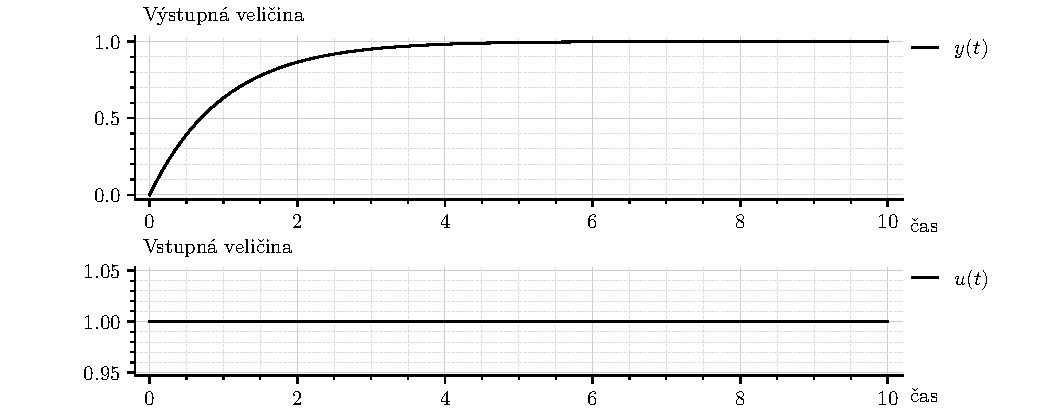
\includegraphics{MRS05_PCH_yu_1.pdf}
	}

	\figcaption{PCH statického systému prvého rádu.}
	\label{PCH SS1R}

\end{center}








\subparagraph{Zostavenie numerickej simulácie -- Python}

Zostavme numerickú simuláciu, ktorej cieľom je získať prechodovú charakteristiku. V nasledujúcom sa využíva Python s~modulmi NumPy a SciPy.

Stavové veličiny samotného lineárneho systému je možné realizovať funkciou:
{\catcode`\-=12
\lstinputlisting[language=Python,
                 caption={Súbor \lstinline{MRS05_kTextu_PCH.py}},
                 label={vypk01},
				 consecutivenumbers=false,
				 linerange=c01-c01,
                 ]{../../PY/MRS05_kTextu_PCH.py}
}
\noindent
kde \lstinline|A| a \lstinline|b| sú samozrejme parametre systému (matica a vektor obsahujúce parametre).

Pre vykonanie simulácie zostavme nasledujúcu funkciu, ktorej hlavná myšlienka je, že vstupný signál systému je po častiach spojitý a~teda jeho zmena je možná s~takpovediac periódou vzorkovania \lstinline|T_s| (viď nasledujúci kód).
{\catcode`\-=12
\lstinputlisting[language=Python,
                 caption={Súbor \lstinline{MRS05_kTextu_PCH.py}},
                 label={vypk02},
				 consecutivenumbers=false,
				 linerange=c02-c02,
                 ]{../../PY/MRS05_kTextu_PCH.py}
}


Prvým nastavením simulácie sú takpovediac časové nastavenia, teda čas začiatku a čas konca a k tomu už uvedená kvázi perióda vzorkovania (skôr logovania/zapisovania), v tomto prípade:
{\catcode`\-=12
\lstinputlisting[language=Python,
                 caption={Súbor \lstinline{MRS05_kTextu_PCH.py}},
                 label={vypk03},
				 consecutivenumbers=false,
				 linerange=c03-c03,
                 ]{../../PY/MRS05_kTextu_PCH.py}
}
\noindent
kde \lstinline|sim_finalIndex| je vlastne počet iterácií \lstinline|for| cyklu tvoriaceho jadro simulačnej funkcie (simulačného skriptu), pozri výpis kódu~\ref{vypk02}.

Ďalším nastavením simulácie je v tomto prípade externý vstupný signál. V každom kroku, v každej iterácii simulácie musí byť dané aká je hodnota tohto signálu.  V tomto prípade realizujeme jednotkový skok, teda:
{\catcode`\-=12
\lstinputlisting[language=Python,
                 caption={Súbor \lstinline{MRS05_kTextu_PCH.py}},
                 % label={vypk01},
				 consecutivenumbers=false,
				 linerange=c04-c04,
                 ]{../../PY/MRS05_kTextu_PCH.py}
}
\noindent



Spustenie simulácie:
{\catcode`\-=12
\lstinputlisting[language=Python,
                 caption={Súbor \lstinline{MRS05_kTextu_PCH.py}},
                 % label={vypk01},
				 consecutivenumbers=false,
				 linerange=c06-c06,
                 ]{../../PY/MRS05_kTextu_PCH.py}
}
\noindent
Výsledok je na obr.~\ref{PCH SS1R}




\subparagraph{Zostavenie numerickej simulácie -- MATLAB/Simulink}

Simulink priamo ponúka prácu s prenosovými funkciami a teda za užívateľa vykoná prevod do opisu v stavovom priestore a vykoná numerickú simuláciu. Pre tento prípad by schéma v simulinku vyzerala nasledovne:

\begin{center}

    \makebox[\textwidth][c]{%
	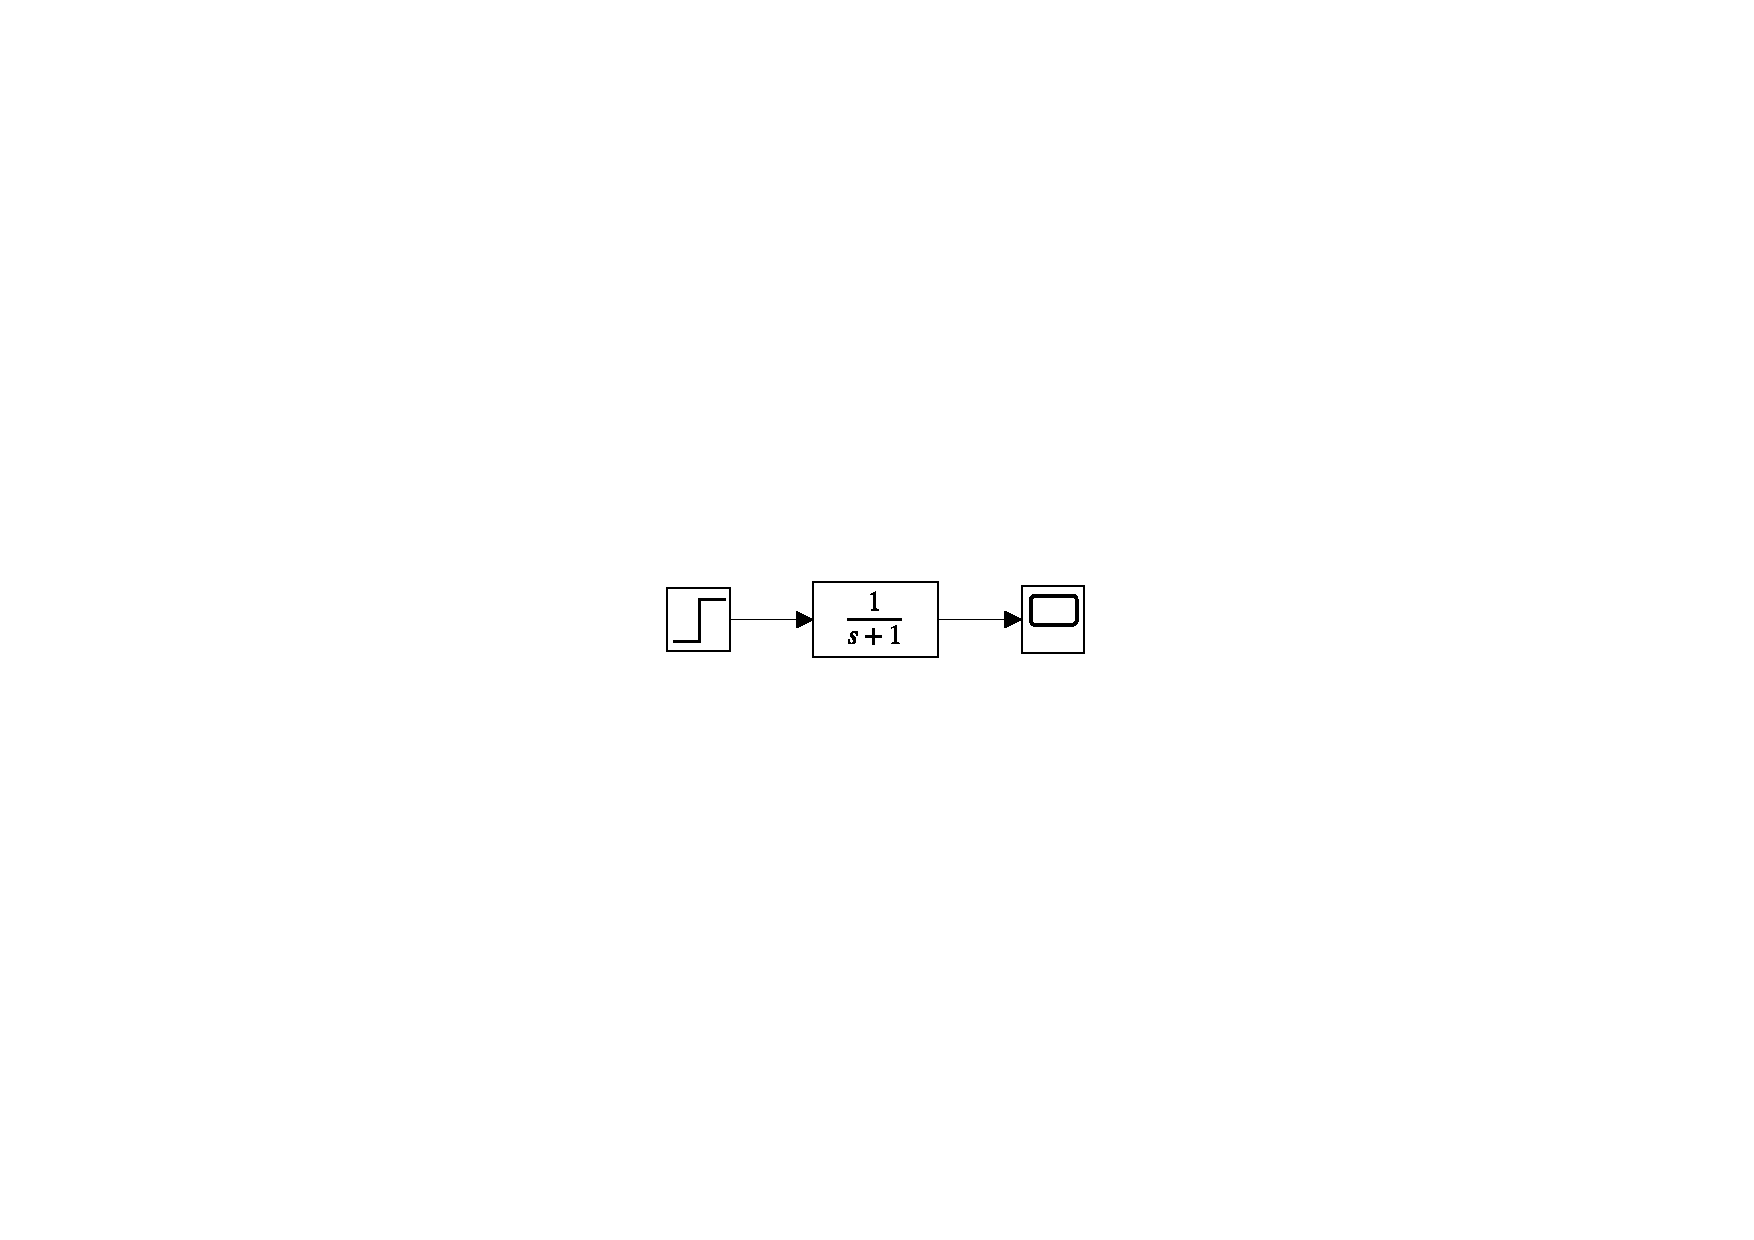
\includegraphics[trim=110mm 95mm 110mm 95mm, clip]{simulinkPCHSS1R.pdf}
	}

    \vspace{-5mm}

	\figcaption{Simulačná schéma pre PCH SS1R}
	\label{sim_PCHSS1R}

    \vspace{-1mm}

\end{center}

V bloku \lstinline|Step| je v tomto prípade nastavený skok v~čase $0$~z~hodnoty $0$~na hodnotu~$1$.

\medskip

S využitím \emph{Control System Toolbox} v MATLABe je možné získať PCH príkazom  \lstinline|step()|. Samozrejme, najprv je potrebné zadefinovať systém, ktorého PCH nás zaujíma, čo je možné v tomto toolboxe priamo vo forme prenosovej funkcie príkazom  \lstinline|tf()|. Teda:
\begin{lstlisting}[language=Matlab,]
G = tf([1], [1, 1])
step(G)
\end{lstlisting}
\noindent
pričom príkaz \lstinline|step()| sa postará o časové nastavenie simulácie (nájde vhodné nastavenie pre ODE solver atď) a priamo vykreslí aj obrázok.











\paragraph{PCH astatického systému prvého rádu (AS1R)}

Pripomeňme, že sa tu zaoberáme prenosovou funkciou v tvare
\begin{align} \label{typ1radtf3}
    G(s) = \frac{b_0}{s}
\end{align}
a po prevode do oppisu v stavovom priestore
\begin{align}
    \dot x_1(t) &= b_0 u(t) \\
    y(t) &= x_1(t)
\end{align}
Zvoľme $b_0 = 1$. A teda (pozri ďalej výpis kódu~\ref{vypk01}):
{\catcode`\-=12
\lstinputlisting[language=Python,
                 caption={Súbor \lstinline{MRS05_kTextu_PCH.py}},
                 label={vypk07},
				 consecutivenumbers=false,
				 linerange=c07-c07,
                 ]{../../PY/MRS05_kTextu_PCH.py}
}
\noindent

Prechodová charakteristika statického systému prvého rádu je na obr.~\ref{PCH AS1R}.

\begin{center}

    \makebox[\textwidth][c]{%
	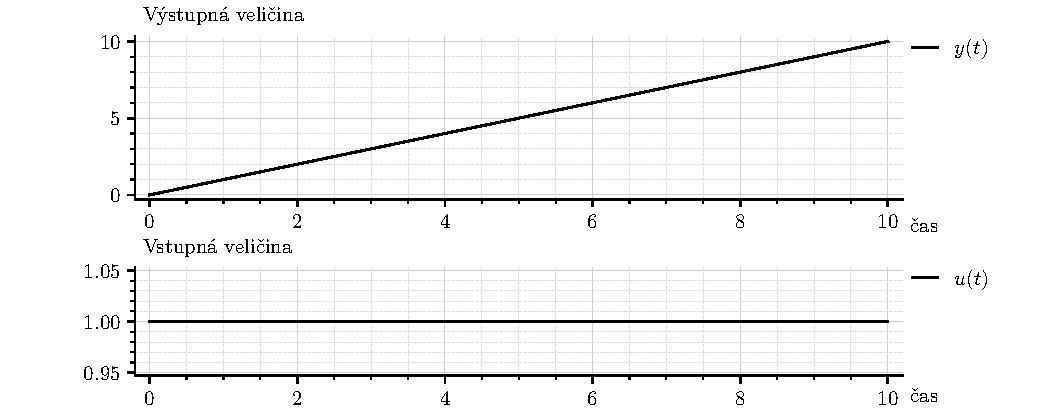
\includegraphics{MRS05_PCH_yu_2.pdf}
	}

	\figcaption{PCH astatického systému prvého rádu.}
	\label{PCH AS1R}

\end{center}





\paragraph{PCH nestabilného statického systému prvého rádu}

Pripomeňme, že  systém v tomto prípade je stabilný ak $a_0 > 0$, nestabilný ak $a_0 < 0$, a ak $a_0 = 0$, tak systém je na hranici stability. Zvoľme preto $a_0 = -1$, v kóde teda:
{\catcode`\-=12
\lstinputlisting[language=Python,
                 caption={Súbor \lstinline{MRS05_kTextu_PCH.py}},
                 label={vypk11},
				 consecutivenumbers=false,
				 linerange=c11-c11,
                 ]{../../PY/MRS05_kTextu_PCH.py}
}
\noindent
Prechodová charakteristika statického systému prvého rádu je na obr.~\ref{PCHnestabilSS1R}. Výstup systému sa neustáli a rastie do nekonečna.

\begin{center}

    \makebox[\textwidth][c]{%
	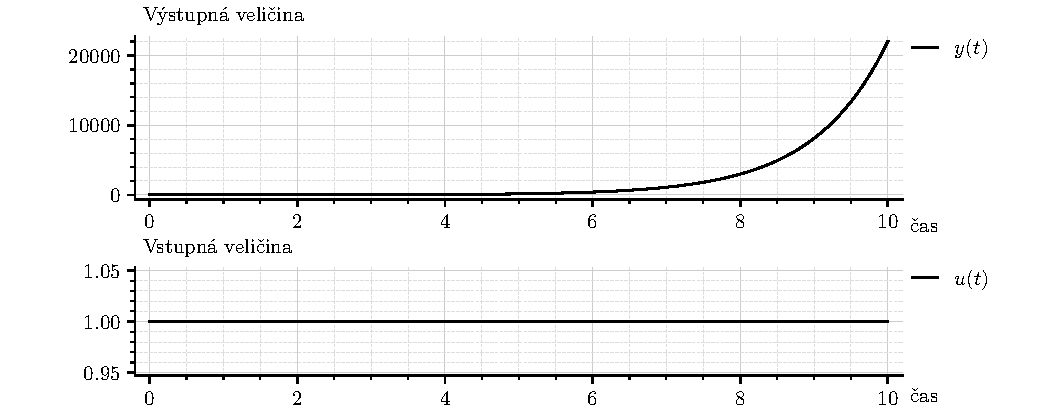
\includegraphics{MRS05_PCH_yu_11.pdf}
	}

	\figcaption{PCH nestabilného statického systému prvého rádu.}
	\label{PCHnestabilSS1R}

\end{center}














\subsubsection{Impulzná charakteristika}

Impulzná charakteristika (ICH) je odpoveď systému na Dirackov impulz (nekonečne krátky impulz s jednokovou plochou).




\paragraph{ICH statického systému prvého rádu (SS1R)}

Pripomeňme, že sa tu zaoberáme prenosovou funkciou v tvare
\begin{align} \label{typ1radtf4}
    G(s) = \frac{b_0}{s + a_0}
\end{align}
Zvoľme $a_0 = 1$, $b_0 = 1$. Impulzná charakteristika statického systému prvého rádu je na obr.~\ref{ICH SS1R}.

\begin{center}

    \makebox[\textwidth][c]{%
	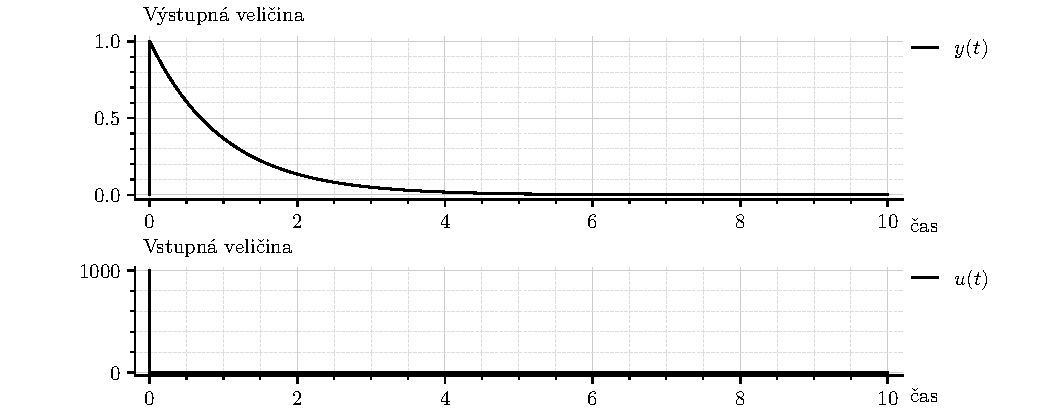
\includegraphics{MRS05_PCH_yu_3.pdf}
	}

	\figcaption{ICH statického systému prvého rádu.}
	\label{ICH SS1R}

\end{center}



\subparagraph{Zostavenie numerickej simulácie -- Python}

Jedinou zmenou oproti predchádzajúcemu čo sa zostavenia simulácie týka je zmena vstupného signálu $u(t)$.

Je potrebné realizovať aproximáciu Dirackovho impulzu. Šírka impulzu je ideálne nekonečne krátka. To je nerealizovateľné. Zvoľme preto najmenšiu možnú šírku impulzu danú kvázi periódou vzorkovania \lstinline|T_s|.

Ďalej je potrebné pri aproximovaní splniť požiadavku, že plocha impulzu má byť jednotková. Ak šírka impulzu má hodnotu \lstinline|T_s|, potom ak výška impulzu bude \lstinline|1/T_s|, výsledná plocha bude jednotková. Teda:
{\catcode`\-=12
\lstinputlisting[language=Python,
                 caption={Súbor \lstinline{MRS05_kTextu_PCH.py}},
                 label={vypk08},
				 consecutivenumbers=false,
				 linerange=c08-c08,
                 ]{../../PY/MRS05_kTextu_PCH.py}
}
\noindent

\subparagraph{Zostavenie numerickej simulácie -- MATLAB/Simulink}

S využitím \emph{Control System Toolbox} v MATLABe je možné získať ICH príkazom  \lstinline|impulse()|. Samozrejme, najprv je potrebné zadefinovať systém, ktorého ICH nás zaujíma, čo je možné v tomto toolboxe priamo vo forme prenosovej funkcie príkazom  \lstinline|tf()|. Teda:
\begin{lstlisting}[language=Matlab,]
G = tf([1], [1, 1])
impulse(G)
\end{lstlisting}
\noindent
pričom príkaz \lstinline|impulse()| priamo vykreslí aj obrázok.


V Simulinku je napríklad možné realizovať aproximáciu Dirackovho impulzu pomocou bloku \lstinline|Step| s nasledovným nastavením:
\begin{center}

    \makebox[\textwidth][c]{%
	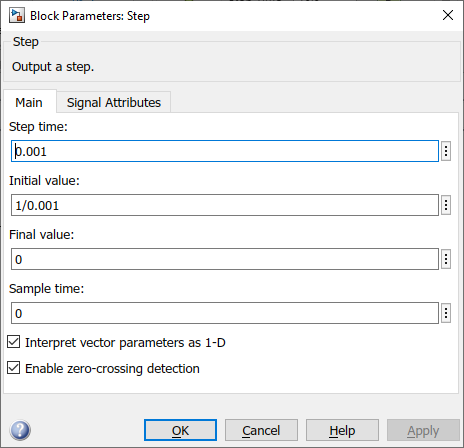
\includegraphics[width=0.68\textwidth]{stepSetup_DiracApprox.png}
	}

	\figcaption{Nastavenie bloku \lstinline|Step|.}
	\label{stepSetup_DiracApprox.png}

\end{center}

Blok je súčasťou schémy:
\begin{center}

    \makebox[\textwidth][c]{%
	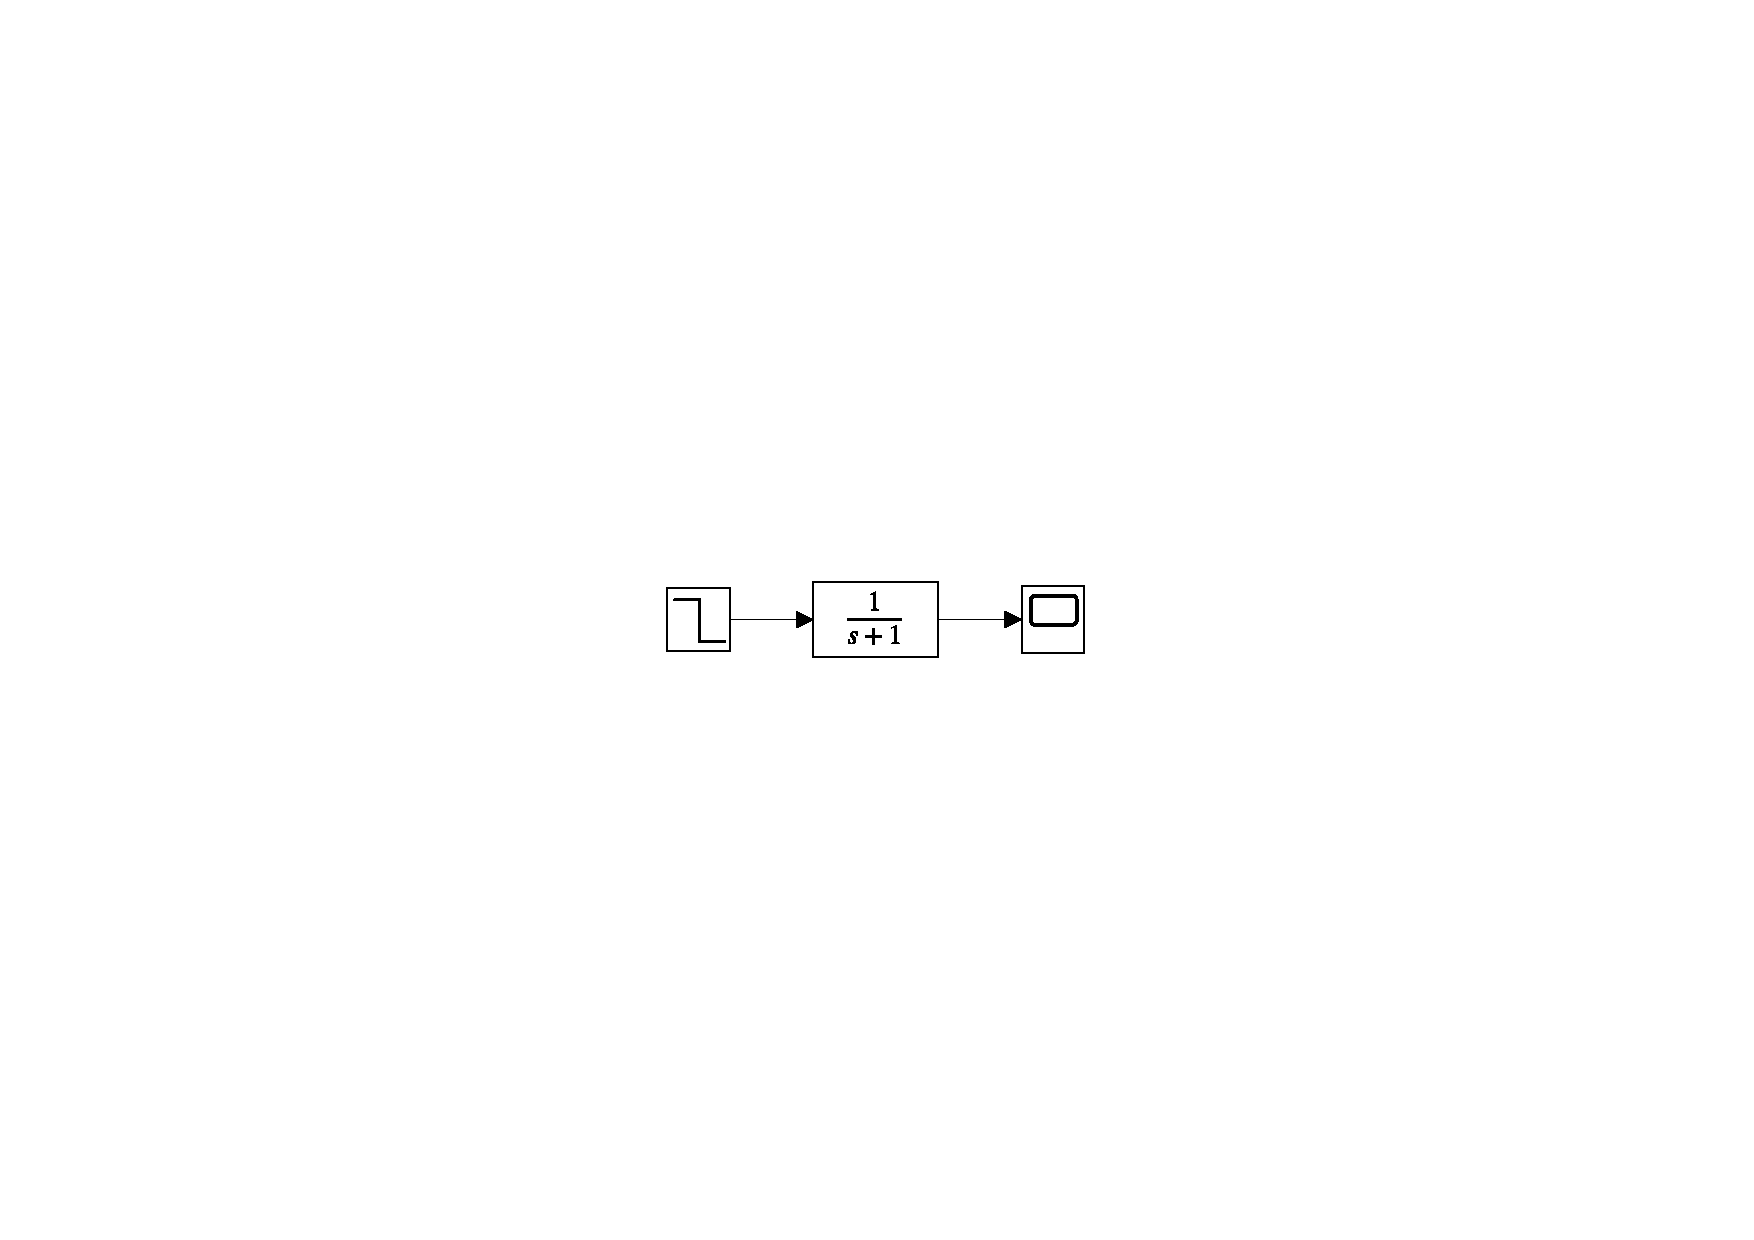
\includegraphics[trim=110mm 95mm 110mm 95mm, clip]{simulinkICHSS1R.pdf}
	}

    \vspace{-5mm}

	\figcaption{Simulačná schéma pre ICH SS1R}
	\label{sim_ICHSS1R}

    \vspace{-1mm}

\end{center}

\paragraph{ICH astatického systému prvého rádu (AS1R)}

Pripomeňme, že sa tu zaoberáme prenosovou funkciou v tvare (zvoľme $b_0 = 1$)
\begin{align} \label{typ1radtf5}
    G(s) = \frac{b_0}{s}
\end{align}
a teda ide o integrátor.

Plocha Dirackovho impulzu je jednotková. Ak privedieme takýto impulz na vstup integrátora, jeho výstupom bude vlastne jednotkový skok. Ak integrálom Dirackovho impulzu je jednokový skok, potom deriváciou jednotkového skoku je Dirackov impulz.


Impulzná charakteristika astatického systému prvého rádu je na obr.~\ref{ICH AS1R}.

\begin{center}

    \makebox[\textwidth][c]{%
	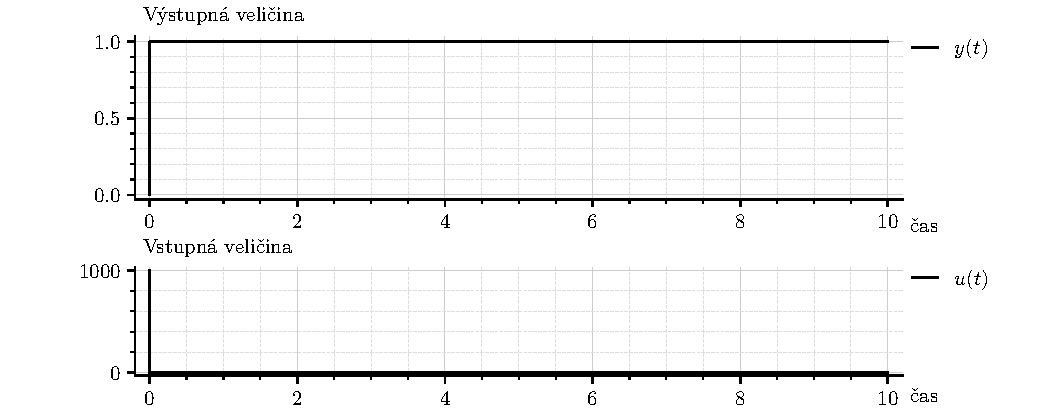
\includegraphics{MRS05_PCH_yu_4.pdf}
	}

	\figcaption{ICH astatického systému prvého rádu.}
	\label{ICH AS1R}

\end{center}








\paragraph{ICH nestabilného statického systému prvého rádu}

Pripomeňme, že  systém v tomto prípade je stabilný ak $a_0 > 0$, nestabilný ak $a_0 < 0$, a ak $a_0 = 0$, tak systém je na hranici stability. Zvoľme preto $a_0 = -1$.

Prechodová charakteristika statického systému prvého rádu je na obr.~\ref{ICHnestabilSS1R}. Vstupný impulz vychýli systém z rovnovážneho stavu a hodnota výstupnej veličiny následne rastie s časom do nekonečna.

\begin{center}

    \makebox[\textwidth][c]{%
	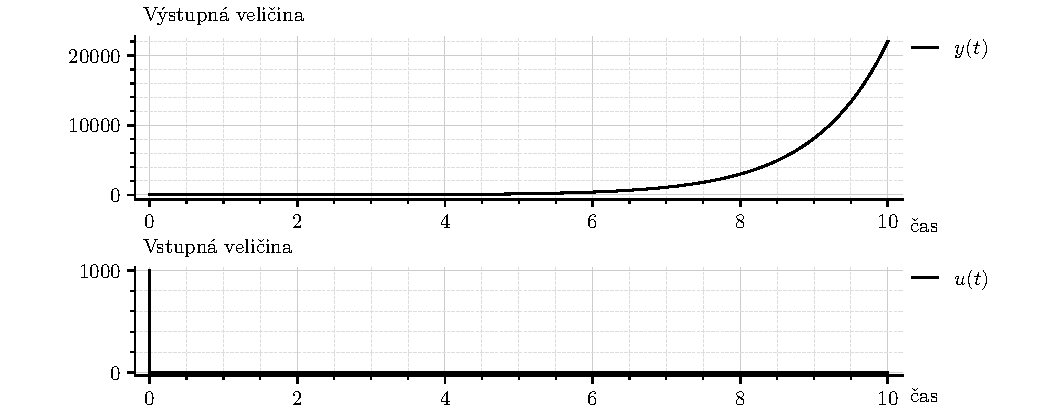
\includegraphics{MRS05_PCH_yu_12.pdf}
	}

	\figcaption{ICH nestabilného statického systému prvého rádu.}
	\label{ICHnestabilSS1R}

\end{center}
















\subsection{Systém nultého rádu}

Stupeň polynómu $A(s)$ môže byť aj $n = 0$. Potom hovoríme o systéme nultého rádu. Prenosová funkcia v tomto prípade je (aj vzhľadom na kauzálnosť, aj vzhľadom na pozitívnu reálnosť)
\begin{align}
    G(s) = \frac{b_0}{a_0}
\end{align}

Hovoriť v tomto prípade o dynamike v podstate nie je možné. Ide tu vo všeobecnosti o zosilňovač, ktorého statické zosilnenie je
\begin{align}
    \frac{y(\infty)}{u(\infty)} = \frac{b_0 }{a_0}
\end{align}
Takýto systém má len statické vlastnosti (statické zosilnenie -- sklon prevodovej charakteristiky). O~dynamických vlastnostiach, v~zmysle astatizmu, stability a~prechodovej charakteristiky tu nemá význam hovoriť.






\subsection{Systém druhého rádu}

Ak stupeň polynómu $A(s)$ je $n = 2$, potom hovoríme, že systém je druhého rádu. Pre kauzálnosť a aj pre pozitívnu reálnosť tu uvažujeme $m<n$ a tak vo všeobecnosti
\begin{align} \label{typ2radtf}
    G(s) = \frac{b_1 s + b_0}{s^2 + a_1 s + a_0}
\end{align}
kde je $A(s)$ bez straty na všeobecnosti uvedený ako monický polynóm.

Obdobne, prenosovou funkciou druhého rádu sú:
\begin{subequations}
    \begin{align}
        G(s) &= \frac{b_0}{s^2 + a_1 s + a_0} \\
        G(s) &= \frac{b_1 s}{s^2 + a_1 s + a_0}
    \end{align}
\end{subequations}


\subsubsection{Prevod na diferenciálnu rovnicu}

Z \eqref{typ2radtf} je zrejmé, že
\begin{align}
    (s^2 + a_1 s + a_0) Y(s) = (b_1 s + b_0) U(s)
\end{align}
a teda
\begin{align} \label{difrovnicanavsimnutie2}
    \ddot y(t) + a_1 \dot y(t) + a_0 y(t) = b_1 \dot u(t) + b_0 u(t)
\end{align}
je zodpovedajúca diferenciálna rovnica. Neznámou je samozrejme časová funkcia $y(t)$ a ako externý vstup je potrebné poznať signál $u(t)$ ale aj jeho časovú deriváciu $\dot u(t)$.




\subsubsection{Prevod do stavového priestoru}

Ide tu vo všeobecnosti o prepis diferenciálnej rovnice vyššieho rádu na sústavu rovníc prvého rádu.

Prevod z prenosovej funkcie na stavový opis nie je jednoznačný. Záleží na voľbe stavových veličín (stavového priestoru). Tu si dovolíme uviesť voľbu stavových veličín tak, že výsledkom je opis systému v tzv. normálnej forme riaditeľnosti.

Prenosová funkcia systému, ktorou sa tu zaoberáme, je v tvare
\begin{align} \label{tfVseob01}
	\frac{Y(s)}{U(s)} = \frac{b_1 s + b_0}{ s^2 + a_1 s + a_0}
\end{align}
Otázka je ako túto prenosovú funkciu previesť na opis v stavovom priestore - ako zvoliť stavové veličiny. Pre prípad, keď je v čitateli len konštanta (systém nemá nuly), je voľba stavových veličín značne intuitívna. Preto napíšme prenosovú funkciu \eqref{tfVseob01} ako dve prenosové funkcie v sérii nasledovne
\begin{align}
	\frac{Z(s)}{U(s)} &= \frac{1}{ s^2 + a_1 s + a_0} \label{tfVseob02a} \\
    \frac{Y(s)}{Z(s)} &= b_1 s + b_0 \label{tfVseob02b}
\end{align}
kde sme zaviedli pomocnú veličinu $Z(s)$, ktorá je obrazom $z(t)$.

Prvú prenosovú funkciu $\eqref{tfVseob02a}$ možno prepísať na diferenciálnu rovnicu druhého rádu v tvare
\begin{align} \label{origdifeqnz}
	\ddot z(t) + a_1 \dot z(t) + a_0 z(t) = u(t)
\end{align}

Túto je možné previesť na sústavu diferenciálnych rovníc prvého rádu - voľbou stavových veličín. Napríklad nech
\begin{align}
	x_1(t) = z(t)
\end{align}
kde $x_1(t)$ je prvá stavová veličina. Potom platí
\begin{align}
	\dot x_1(t) = \dot z(t)
\end{align}
Druhú stavovú veličinu zvoľme
\begin{align}
	x_2(t) = \dot z(t)
\end{align}
a teda
\begin{align} \label{zardrufdifr}
	\dot x_2(t) = \ddot z(t)
\end{align}
V tomto bode môžeme ľahko písať
\begin{align}
	\dot x_1(t) &= x_2(t)
\end{align}
To je prvá diferenciálna rovnica! Obsahuje len novo zavedené stavové veličiny ($x_1(t)$ a~$x_2(t)$). Druhá diferenciálna rovnica je vlastne \eqref{zardrufdifr}. Avšak, vieme signál $\ddot z(t)$ vyjadriť len pomocou novo zavedených stavových veličín? Vieme. Z \eqref{origdifeqnz} je zrejmé, že
\begin{align}
	\ddot z(t) = - a_1 \dot z(t) - a_0 z(t) + u(t) = - a_1 x_2(t) - a_0 x_1(t) + u(t)
\end{align}
takže \eqref{zardrufdifr} je
\begin{align}
	\dot x_2(t) =  - a_1 x_2(t) - a_0 x_1(t) + u(t)
\end{align}
a to je druhá diferenciálna rovnica\ldots

Obe rovnice spolu:
\begin{align}
    \dot x_1(t) &= x_2(t) \\
	\dot x_2(t) &=  - a_1 x_2(t) - a_0 x_1(t) + u(t)
\end{align}
A v maticovom zápise:
\begin{align}
	\begin{bmatrix}
    	  \dot x_1(t) \\
		  \dot x_2(t)
 	\end{bmatrix}
	&=
	\begin{bmatrix}
    	0 & 1 \\
    	- a_0 & - a_1
  	\end{bmatrix}
    \begin{bmatrix}
    	  x_1(t) \\
		  x_2(t)
 	\end{bmatrix}
    +
    \begin{bmatrix}
    	  0 \\
		  1
 	\end{bmatrix}
    u(t)
\end{align}


Vráťme sa k prenosovej funkcii \eqref{tfVseob02b}. Túto možno napísať ako diferenciálnu rovnicu v tvare
\begin{align} \label{difrov2}
    y(t) = b_1 \dot z(t) + b_0 z(t)
\end{align}
Avšak, my sme už urobili voľbu takú, že $\dot z(t) = x_2(t)$ a $z(t)= x_1(t)$. Takže diferenciálnu rovnicu \eqref{difrov2} môžme písať ako
\begin{align}
    y(t) = b_1 x_2(t) + b_0 x_1(t)
\end{align}
alebo v maticovom tvare
\begin{align}
	y(t)
	&=
	\begin{bmatrix}
    	b_0 & b_1 \\
  	\end{bmatrix}
    \begin{bmatrix}
    	  x_1(t) \\
		  x_2(t)
 	\end{bmatrix}
\end{align}



Celý systém s novo zavedenými stavovými veličinami teda je v tvare
\begin{align}
	\begin{bmatrix}
    	  \dot x_1(t) \\
		  \dot x_2(t)
 	\end{bmatrix}
	&=
	\begin{bmatrix}
    	0 & 1 \\
    	- a_0 & - a_1
  	\end{bmatrix}
    \begin{bmatrix}
    	  x_1(t) \\
		  x_2(t)
 	\end{bmatrix}
    +
    \begin{bmatrix}
    	  0 \\
		  1
 	\end{bmatrix}
    u(t)
    \\
    y(t)
    &=
    \begin{bmatrix}
        b_0 & b_1 \\
    \end{bmatrix}
    \begin{bmatrix}
          x_1(t) \\
          x_2(t)
    \end{bmatrix}
\end{align}
a ak označíme stavový vektor ako $x(t) = \begin{bmatrix} x_1(t) & x_2(t) \end{bmatrix}^\naT$, potom je systém v známom tvare
\begin{subequations} \label{susDifRovnicPreODE}
    \begin{align}
    	\dot x(t) &= A x(t) + b u(t) \\
        y(t) &= c^\naT x(t)
    \end{align}
\end{subequations}
kde matica $A$ a vektory $b$ a $c$ sú zrejmé\ldots




\subsubsection{Statické zosilnenie}

Ak žiadny z pólov systému nie je nulový, potom hovoríme, že systém je statický. To znamená, že je možné určiť jeho statické zosilnenie. Statické zosilnenie je pomer výstupu ku vstupu v ustálenom stave.

V ustálenom stave sa signály nemenia, to znamená, že ich časová derivácie sú nulové. Všimnime si diferenciálnu rovnicu \eqref{difrovnicanavsimnutie2}. V ustálenom stave sú $\ddot y(\infty) = 0$ a~$\dot y(\infty) = 0$, kde $\infty$ symbolizuje čas, v ktorom sú už signály ustálené. Zároveň aj $\dot u(\infty) = 0$. Teda
\begin{align}
    a_0 y(\infty) =  b_0 u(\infty)
\end{align}
Pomer výstupu ku vstupu je
\begin{align}
    \frac{y(\infty)}{u(\infty)} = \frac{b_0 }{a_0}
\end{align}
čo je statické zosilnenie systému. Konvenciou je vo všeobecnosti uvažovať, že vstup je „jednotkový“, jednoducho, že $u(\infty) = 1$ a teda sa píše $y(\infty) = \frac{b_0 }{a_0}$, ale stale sa tým myslí statické zosilnenie systému.

K rovnakému záveru prídeme, ak by sme uvažovali konštantný, ustálený signál na vstupe, a to vo všeobecnosti, teda $u(t) = 1$. To je jednotkový skok a teda $U(s) = \frac{1}{s}$. Potom
\begin{align}
    Y(s) =  \frac{b_1 s + b_0}{s^2 + a_1 s + a_0} \frac{1}{s}
\end{align}
Konečná hodnota tohto obrazu signálu ($Y(s)$ je obrazom $y(t)$), je hodnota na, ktorej sa výstup systému potenciálne ustáli (samozrejme, ak sa vôbec ustáli). S využitím vety o konečnej hodnote:
\begin{subequations}
\begin{align}
    y(\infty) &= \lim_{s \to 0} s \left(  \frac{b_1 s + b_0}{s^2 + a_1 s + a_0} \frac{1}{s} \right) \\
    y(\infty) &= \lim_{s \to 0} \left(  \frac{b_1 s + b_0}{s^2 + a_1 s + a_0}  \right) \\
    y(\infty) &=  \frac{b_0}{a_0}
\end{align}
\end{subequations}







\subsubsection{Astatizmus}

Ak je jeden z pólov systému nulový, hovoríme, že systém je astatický („obsahuje astatizmus“). Ak práve jeden pól je nulový, hovoríme o astatizme prvého rádu. Ak sú dva póly nulové, potom ide o astatizmus druhého rádu, atď.

V tomto prípade máme dva póly. Označme $p_1$ a $p_2$. Ak je jeden z nich nulový, $p_1 = 0$, potom
\begin{align}
    A(s) = (s - p_1)(s - p_2) = (s -0)(s - p_2) = s(s - p_2)
\end{align}
Prenosová funkcia systému druhého rádu s astatizmom prvého rádu by teda mohla byť v tvare
\begin{subequations}
    \begin{align}
        G(s) &= \frac{b_1 s + b_0}{s(s - p_2)} \\
        G(s) &= \frac{b_0}{s(s - p_2)}
        % G(s) &= \frac{b_1 s}{s(s - p_2)}
    \end{align}
\end{subequations}
Všimnime si, že ak by $G(s) = \frac{b_1 s}{s(s - p_2)}$ potom je to vlastne $G(s) = \frac{b_1}{(s - p_2)}$, a~teda nejde o~systém druhého rádu\footnote{Krátime tu vo všeobecnosti polynómy a je potrebné to zohľadniť z matematického hľadiska („deliť polynómom“ nie je vždy možné)}.

Ak by boli oba póly nulové, teda $A(s) = s^2$, potom prenosová funkcia systému druhého rádu s astatizmom druhého rádu by mohla byť v tvare
\begin{subequations}
    \begin{align}
        G(s) &= \frac{b_1 s + b_0}{s^2} \\
        G(s) &= \frac{b_0}{s^2} \label{integratordvojitz}
    \end{align}
\end{subequations}

Mimochodom, prenosová funkcia \eqref{integratordvojitz} je vlastne dvojitý integrátor.



\subsubsection{Stabilita}

Stabilita systému je daná koreňmi charakteristického polynómu $A(s)$, v tomto prípade
\begin{align}
    A(s) = s^2 + a_1 s + a_0
\end{align}
Tento polynóm má dva korene. Môžu to byť:
\begin{itemize}[leftmargin=0pt, labelsep=3mm, itemsep=0pt]
    \item dve rôzne reálne čísla (imaginárna časť čísla je nulová),
    \item jedno reálne číslo, ktoré je dvojnásobným koreňom,
    \item alebo dve komplexné čísla, ktoré sú však navzájom komplexne združené.
\end{itemize}
V každom prípade však platí, že systém je stabilný vtedy, a len vtedy, ak reálne časti pólov sú záporné (v ľavej polrovine komplexnej roviny).

Ak aspoň jeden koreň leží na imaginárnej osi (reálna časť koreňa je nulová), potom hovoríme, že systém je na hranici stability.

Ak aspoň jeden koreň má reálnu časť kladnú, potom je systém nestabilný.








\subsubsection{Prechodová a impulzná charakteristika}



\paragraph{Statický systém druhého rádu (SS2R), prípad $B(s) = b_0$}

V prvom rade uvažujme prípad, keď dynamiku systému určujú len póly systému, teda prenosová funkcia je v tvare
\begin{align}
    G(s) =  \frac{b_0}{s^2 + a_1 s + a_0}
\end{align}
Polynóm $B(s) = b_0$ je nultého stupňa, teda systém nemá žiadne nuly. Označme póly systému $p_1$ a $p_2$. Zvoľme prípad, keď sú dva nezávislé reálne póly, teda napr. $p_1 = -1$ a $p_2 = -2$. Parameter $b_0$ zvoľme tak, že statické zosilnenie systému bude jednotkové, teda $b_0 = a_0$.

Vzhľadom na implementáciu numerickej simulácie uvedenú v predchádzajúcom, pozri výpis kódu~\ref{vypk02}, parametre systému sú
{\catcode`\-=12
\lstinputlisting[language=Python,
                 caption={Súbor \lstinline{MRS05_kTextu_PCH.py}},
                 label={vypk31},
				 consecutivenumbers=false,
				 linerange=c31-c31,
                 ]{../../PY/MRS05_kTextu_PCH.py}
}
\noindent
Výsledná prechodová charakteristika je na obr.~\ref{PCHSS2R_b0} a výsledná impulzná charakteristika je na na obr.~\ref{ICHSS2R_b0}.


\begin{center}

    \makebox[\textwidth][c]{%
	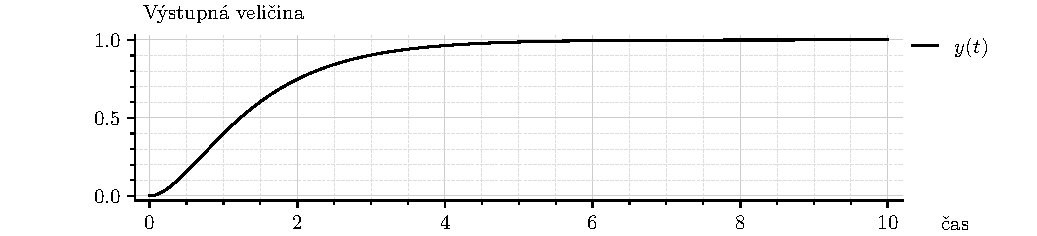
\includegraphics{MRS05_PCH_len_y_31.pdf}
	}

	\figcaption{PCH statického systému druhého rádu (SS2R), $G(s) =  \frac{2}{s^2 + 3 s + 2}$}
	\label{PCHSS2R_b0}

\end{center}

\begin{center}

    \makebox[\textwidth][c]{%
	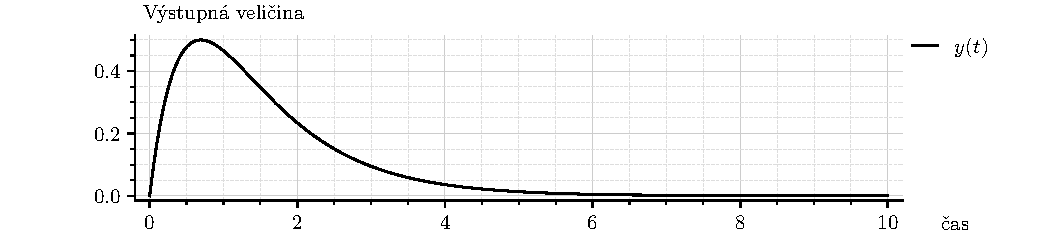
\includegraphics{MRS05_PCH_len_y_311.pdf}
	}

	\figcaption{ICH statického systému druhého rádu (SS2R), $G(s) =  \frac{2}{s^2 + 3 s + 2}$}
	\label{ICHSS2R_b0}

\end{center}



Zvoľme prípad, keď sú jeden viacnásobný koreň, teda napr. $p_1 = -1$ a $p_2 = -1$, výsledná prechodová charakteristika je na obr.~\ref{PCHSS2R_b0_viacn}, výsledná impulzná charakteristika je na obr.~\ref{ICHSS2R_b0_viacn}.

\begin{center}

    \makebox[\textwidth][c]{%
	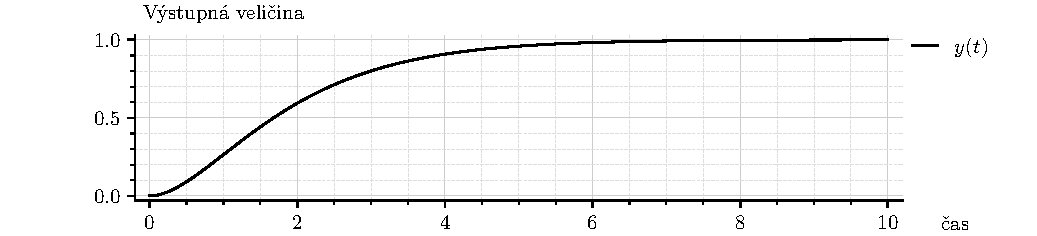
\includegraphics{MRS05_PCH_len_y_32.pdf}
	}

	\figcaption{PCH statického systému druhého rádu (SS2R), $G(s) =  \frac{1}{s^2 + 2 s + 1}$}
	\label{PCHSS2R_b0_viacn}

\end{center}

\begin{center}

    \makebox[\textwidth][c]{%
	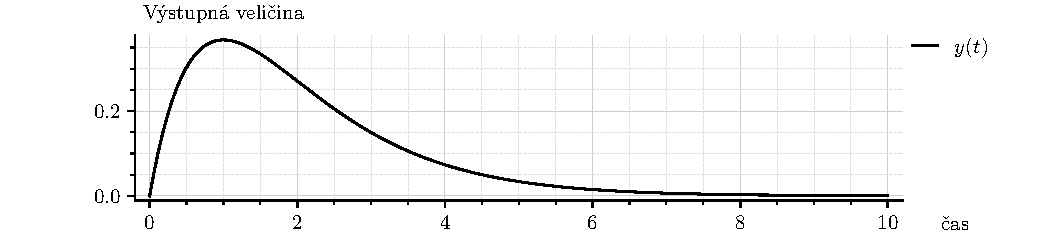
\includegraphics{MRS05_PCH_len_y_321.pdf}
	}

	\figcaption{ICH statického systému druhého rádu (SS2R), $G(s) =  \frac{1}{s^2 + 2 s + 1}$}
	\label{ICHSS2R_b0_viacn}

\end{center}


Ak by sme chceli póly systému, ktoré sú navzájom komplexne združenými číslami, potom je v prípade systému druhého rádu výhodné uvažovať charakteristický polynóm v tvare
\begin{align}
    A(s) = s^2 + 2 \beta \omega_0 s + \omega_0^2
\end{align}
kde $\beta$ a $\omega_0$ sú parametre, pričom $\beta$ sa nazýva koeficient tlmenia a $\omega_0$ sa nazýva vlastná frekvecnia systému. Uvedené označovanie a forma polynómu $A(s)$ vyplývajú z konvencií pri opise oscilácií ako dynamického deja (diferenciálne rovnice tlmených oscilátorov). Ak je parameter $\beta < 1$, potom korene $A(s)$ sú komplexne združené čísla. Ak je parameter $\beta \geq 1$, potom korene $A(s)$ sú reálne.

Zvoľme $\beta = 0.5$ a $\omega_0 = 3$, teda
{\catcode`\-=12
\lstinputlisting[language=Python,
                 caption={Súbor \lstinline{MRS05_kTextu_PCH.py}},
                 label={vypk33},
				 consecutivenumbers=false,
				 linerange=c33-c33,
                 ]{../../PY/MRS05_kTextu_PCH.py}
}
\noindent
Výsledná prechodová charakteristika je na obr.~\ref{PCHSS2R_b0_kmit} a impulzná charakteristika na obr.~\ref{ICHSS2R_b0_kmit}.


\begin{center}

    \makebox[\textwidth][c]{%
	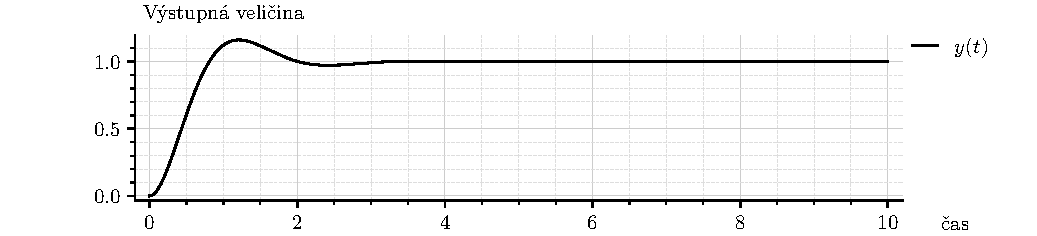
\includegraphics{MRS05_PCH_len_y_33.pdf}
	}

	\figcaption{PCH statického systému druhého rádu (SS2R), $G(s) =  \frac{9}{s^2 + 3 s + 9}$}
	\label{PCHSS2R_b0_kmit}

\end{center}


\begin{center}

    \makebox[\textwidth][c]{%
	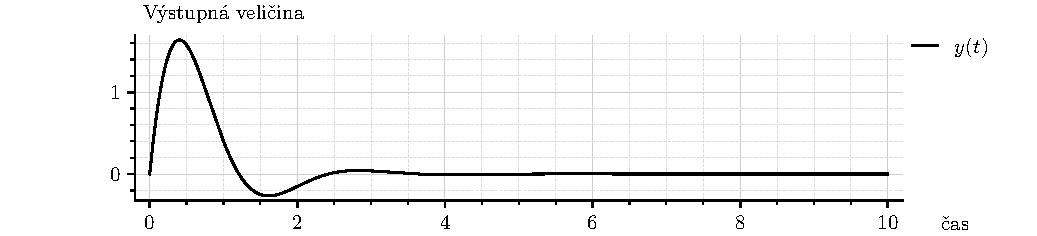
\includegraphics{MRS05_PCH_len_y_331.pdf}
	}

	\figcaption{ICH statického systému druhého rádu (SS2R), $G(s) =  \frac{9}{s^2 + 3 s + 9}$}
	\label{ICHSS2R_b0_kmit}

\end{center}

Ako bolo uvedené, $\beta$ sa nazýva koeficient tlmenia. Ponechajme voľbu $\omega_0 = 3$ a skúmajme vplyv parametra $\beta$ na prechodovú (obr.~\ref{PCHSS2R_b0_kmit_x3}) a impulznú (obr.~\ref{ICHSS2R_b0_kmit_x3}) charakteristiku.

\begin{center}

    \makebox[\textwidth][c]{%
	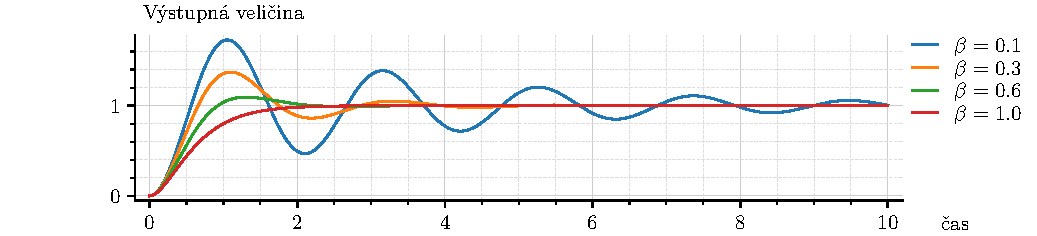
\includegraphics{MRS05_PCH_len_yx3_1.pdf}
	}

	\figcaption{PCH statického systému druhého rádu (SS2R).}
	\label{PCHSS2R_b0_kmit_x3}

\end{center}


\begin{center}

    \makebox[\textwidth][c]{%
	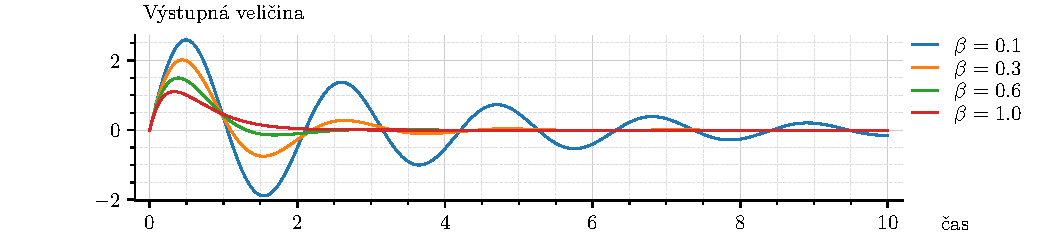
\includegraphics{MRS05_PCH_len_yx3_2.pdf}
	}

	\figcaption{ICH statického systému druhého rádu (SS2R).}
	\label{ICHSS2R_b0_kmit_x3}

\end{center}






\paragraph{Statický systém druhého rádu (SS2R), prípad systému s nulou ($B(s) = b_1 s + b_0$, $B(s) = b_1 s$)}

Je zrejmé, že v prípade ak polynóm $B(s)$ je v tvare $B(s) = b_1 s + b_0$ alebo $B(s) = b_1 s$ má to vplyv na dynamiku systému.

Napríklad, pre polynóm $A(s)$ uvažujme situáciu rovnakú ako na obr.~\ref{PCHSS2R_b0} a~obr.~\ref{ICHSS2R_b0}, teda póly sysému sú $p_1 = -1$ a $p_2 = -2$, teda $A(s) = s^2 + 3s + 2$. Polynóm $B(s)$ zvoľme $B(s) = 3 s + 2$. Výsledná prechodová charakteristika je na obr.~\ref{PCHSS2R_B} a výsledná impulzná charakteristika je na na obr.~\ref{ICHSS2R_B}. V tomto prípade je nula systému, označme ju $z_1$, v bode $z_1 = -\frac{2}{3}$ a teda táto nula sa nezhoduje so žiadnym pólom.


\begin{center}

    \makebox[\textwidth][c]{%
	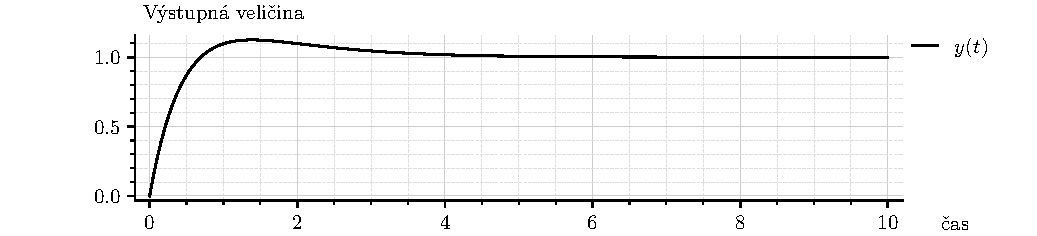
\includegraphics{MRS05_PCH_len_y_41.pdf}
	}

	\figcaption{PCH statického systému druhého rádu (SS2R), $G(s) =  \frac{3 s + 2}{s^2 + 3 s + 2}$}
	\label{PCHSS2R_B}

\end{center}

\begin{center}

    \makebox[\textwidth][c]{%
	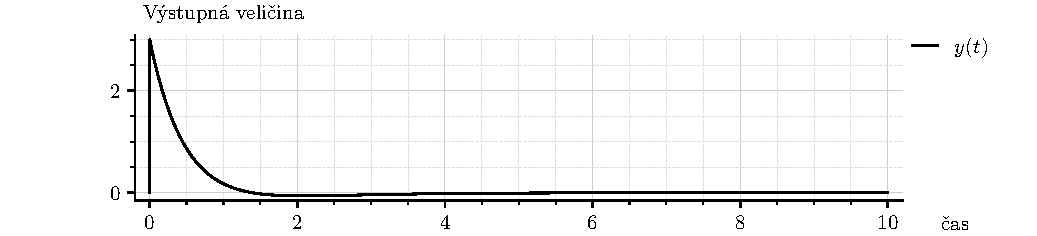
\includegraphics{MRS05_PCH_len_y_411.pdf}
	}

	\figcaption{ICH statického systému druhého rádu (SS2R), $G(s) =  \frac{3 s + 2}{s^2 + 3 s + 2}$}
	\label{ICHSS2R_B}

\end{center}

Ak by sa nula zhodovala s pólom, teda napr bola by to $z_1 = -1$, potom by sme mali $G(s) =  \frac{s + 1}{s^2 + 3 s + 2}$, čo je možné zapísať aj ako $G(s) =  \frac{(s + 1)}{(s+1)(s+2)} =  \frac{1}{(s+2)}$, čo je systém prvého rádu.

Pre úplnosť uvažujme tu aj prípad keď $B(s) = b_1 s$. Zvoľme napríklad $b_1 = 3$. Zachovávame $A(s) = s^2 + 3 s + 2$. Všimnime si, že teraz máme $b_0 = 0$. To znamená, že zosilnenie systému, teda hodnota $b_0/a_0$ bude v tomto prípade nulové. Pre PCH to znamená, že sa ustáli na nule. Prechodová charakteristika pre tento prípad je na obr.~\ref{PCHSS2R_Bs} a impulzná charakteristika je na obr.~\ref{ICHSS2R_Bs}.

\begin{center}

    \makebox[\textwidth][c]{%
	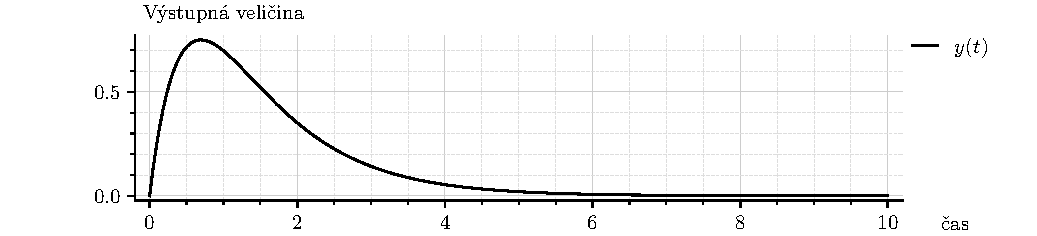
\includegraphics{MRS05_PCH_len_y_51.pdf}
	}

	\figcaption{PCH statického systému druhého rádu (SS2R), $G(s) =  \frac{3s}{s^2 + 3 s + 2}$}
	\label{PCHSS2R_Bs}

\end{center}

\begin{center}

    \makebox[\textwidth][c]{%
	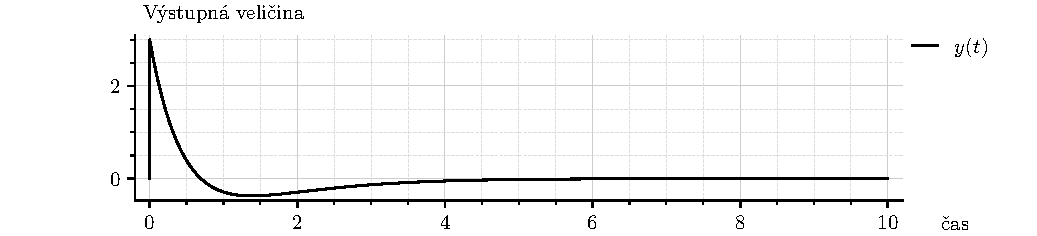
\includegraphics{MRS05_PCH_len_y_511.pdf}
	}

	\figcaption{ICH statického systému druhého rádu (SS2R), $G(s) =  \frac{3s}{s^2 + 3 s + 2}$}
	\label{ICHSS2R_Bs}

\end{center}




\paragraph{Astatický systém druhého rádu (SS2R), prípad $B(s) = b_0$}

Ak je jeden z pólov systému nulový, hovoríme, že systém je astatický („obsahuje astatizmus“). Ak práve jeden pól je nulový, hovoríme o astatizme prvého rádu. Zvoľme tu $B(s) = 1$ a póly $p_1 = -1$ a $p_2 = 0$. Teda $A(s) = s^2 + s$.

Prechodová charakteristika pre tento prípad je na obr.~\ref{PCHAS2R_B} a impulzná charakteristika je na obr.~\ref{ICHAS2R_B}.

\begin{center}

    \makebox[\textwidth][c]{%
	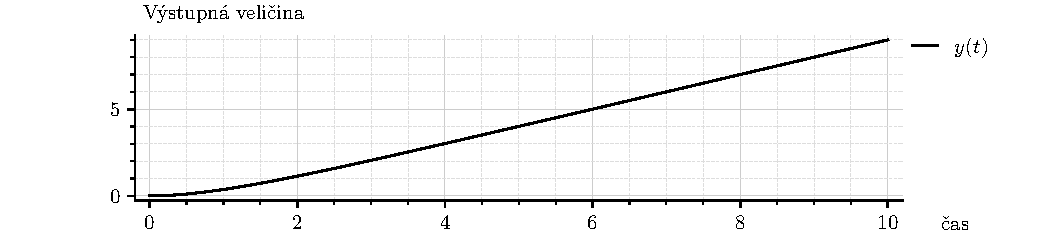
\includegraphics{MRS05_PCH_len_y_61.pdf}
	}

	\figcaption{PCH astatického systému druhého rádu (AS2R), $G(s) = \frac{1}{s^2 + s}$}
	\label{PCHAS2R_B}

\end{center}

\begin{center}

    \makebox[\textwidth][c]{%
	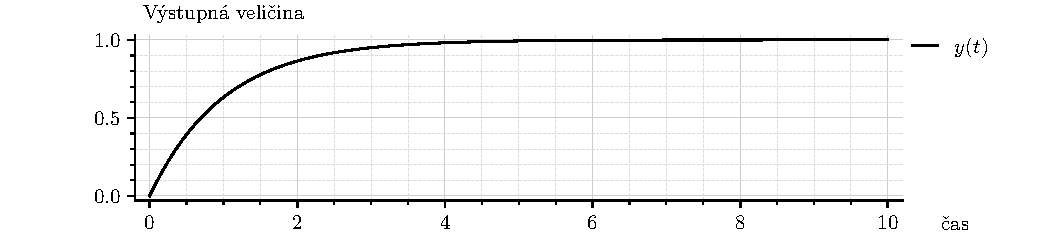
\includegraphics{MRS05_PCH_len_y_611.pdf}
	}

	\figcaption{ICH astatického systému druhého rádu (AS2R), $G(s) = \frac{1}{s^2 + s}$}
	\label{ICHAS2R_B}

\end{center}

Prípadne by sme mohli mať póly $p_1 = 0$ a $p_2 = 0$. Teda $A(s) = s^2$. Prechodová charakteristika pre tento prípad je na obr.~\ref{PCHAS2R_B2} a impulzná charakteristika je na obr.~\ref{ICHAS2R_B2}.

\begin{center}

    \makebox[\textwidth][c]{%
	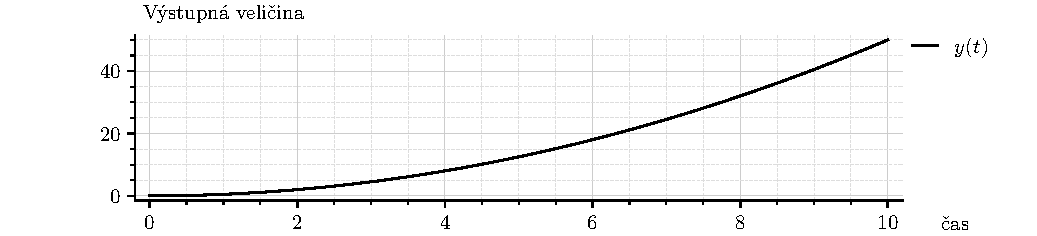
\includegraphics{MRS05_PCH_len_y_71.pdf}
	}

	\figcaption{PCH astatického systému druhého rádu (AS2R), $G(s) = \frac{1}{s^2}$}
	\label{PCHAS2R_B2}

\end{center}

\begin{center}

    \makebox[\textwidth][c]{%
	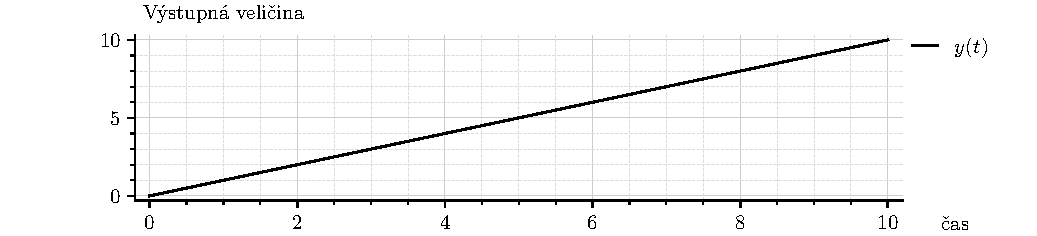
\includegraphics{MRS05_PCH_len_y_711.pdf}
	}

	\figcaption{ICH astatického systému druhého rádu (AS2R), $G(s) = \frac{1}{s^2}$}
	\label{ICHAS2R_B2}

\end{center}


\paragraph{Astatický systém druhého rádu (AS2R), prípad systému s nulou ($B(s) = b_1 s + b_0$)}

Azda len pre zaujímavosť tu zvoľme $B(s) =  s + 1$, pritom ponechajme póly $p_1 = 0$ a~$p_2 = 0$, teda $A(s) = s^2$.  Prechodová charakteristika pre tento prípad je na obr.~\ref{PCHAS2R_B3} a~impulzná charakteristika je na obr.~\ref{ICHAS2R_B3}.

\begin{center}

    \makebox[\textwidth][c]{%
	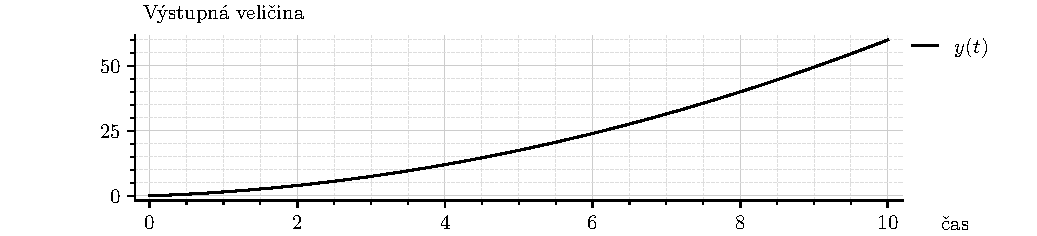
\includegraphics{MRS05_PCH_len_y_81.pdf}
	}

	\figcaption{PCH astatického systému druhého rádu (AS2R), $G(s) = \frac{s + 1}{s^2}$}
	\label{PCHAS2R_B3}

\end{center}

\begin{center}

    \makebox[\textwidth][c]{%
	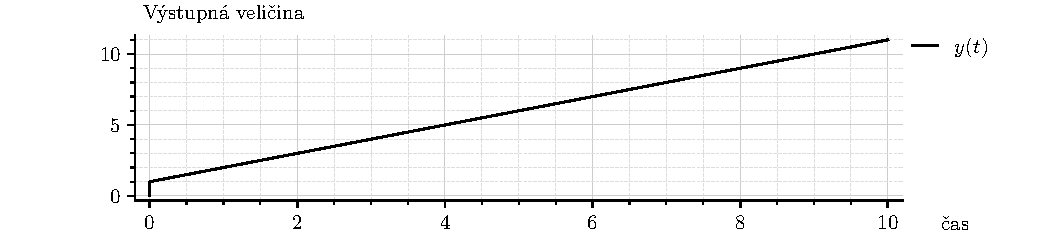
\includegraphics{MRS05_PCH_len_y_811.pdf}
	}

	\figcaption{ICH astatického systému druhého rádu (AS2R), $G(s) = \frac{s + 1}{s^2}$}
	\label{ICHAS2R_B3}

\end{center}












% \pagebreak

\section{Algebra prenosových funkcií {\color{Gray} \small (pripravuje sa)}}

TODO\ldots

\medskip

\noindent
Pozri časť 9.4 v~\cite{AsM08se}.
















\section{Cvičenie šieste}

Priestor pre oboznámenie sa s typickým „control toolboxom“ - sadou výpočtových nástrojov pre oblasť návrhu riadiacich systémov (napr. Control System Toolbox v~MATLABe).

\subsection{Úlohy cvičenia}

\begin{enumerate}[leftmargin=0pt, labelsep=4mm, itemsep=0pt]

	\item Vypočítajte póly lineárnych dynamických systémov daných prenosovými funkciami.

	\item Nakreslite prechodové charakteristiky lineárnych dynamických systémov daných prenosovými funkciami.

	\item Nakreslite impulzné charakteristiky lineárnych dynamických systémov daných prenosovými funkciami.

\end{enumerate}


\noindent
Lineárne dynamické systémy sú pre toto cvičenie definované prenosovou funkciou so všeobecnými parametrami v tvare
\begin{equation*}
	G(s) = \frac{b_2 s^2 + b_1 s + b_0}{a_3 s^3 + a_2 s^2 + a_1 s + a_0} e^{-Ds}
\end{equation*}
a tabuľkou, v ktorej sú uvedené hodnoty parametrov jednotlivých systémov:



\bigskip




\begin{centering}
\catcode`\-=12

\begin{tabular*}{1.0\columnwidth}{ @{\extracolsep{\fill}} c  c c c c c c c c c c }
\toprule
\multicolumn{1}{l}{Systém} & \multicolumn{8}{l}{Parameter} & \multicolumn{1}{l}{Obrázok}   \\
 & $b_2$ & $b_1$ & $b_0$ & $a_3$ & $a_2$ & $a_1$ & $a_0$ & $D$ & \multicolumn{1}{c}{PCH}    \\
\midrule
$1$. & & & $1$ & & & $1$ & $1$ & & \multirow{4}{*}[-6pt]{\rotatebox{90}{Obr. 1.}}   \\
$2$. & & & $1$ & & & $1$ & $1$ & $5$ &   \\
$3$. & & & $0,1$ & & & $1$ & $0$ & &   \\
$4$. & & & $0,1$ & & & $1$ & $0$ & $3$ &   \\ \cmidrule{10-10}
$5$. & & $1$ & $1$ & & & $3$ & $1$ & & \multirow{2}{*}[0pt]{\rotatebox{90}{2.}}  \\
$6$. & & $1$ & $-1$ & & & $3$ & $1$ & & & \\ \cmidrule{10-10}
$7$. & & & $0,5$ & & $1$ & $2$ & $1$ & &  \multirow{4}{*}[0pt]{\rotatebox{90}{Obr. 3.}}  \\
$8$. & & & $0,5$ & & $1$ & $1$ & $1$ & & & \\
$9$. & & & $0,5$ & & $1$ & $0,2$ & $1$ & & & \\
$10$. & & & $0,5$ & & $1$ & $0$ & $1$ & &  & \\ \cmidrule{10-10}
$11$. & & & $0,2$ & & $1$ & $1$ & $0$ & & \multirow{3}{*}[-3pt]{\rotatebox{90}{Obr. 4.}}   \\
$12$. & & & $0,2$ & & $1$ & $0$ & $0$ & &   \\
$13$. & & & $0,2$ & & $1$ & $0$ & $0$ & $4$ &   \\ \cmidrule{10-10}
$14$. & $1$ & $2$ & $2$ & $1$ & $0,3$ & $4,03$ & $0,401$ &  & \multirow{2}{*}[0pt]{\rotatebox{90}{5.}}   \\
$15$. & $1$ & $2$ & $2$ & $1$ & $0,3$ & $4,03$ & $0,401$ & $6$ &  \\
\bottomrule
\end{tabular*}
\end{centering}

\medskip

\noindent
Tabuľka určuje aj číslo obrázka, do ktorého nakreslite príslušnú charakteristiku (PCH). Niektoré charakteristiky sú na spoločnom obrázku.














\section{Otázky a úlohy}

\begin{enumerate}[leftmargin=0pt, labelsep=3mm, itemsep=0pt]


    \item Pre lineárny dynamický systém zadaný diferenciálnou rovnicou nájdite jeho prenosovú funkciu.

	\item Pre dynamický systém opísaný pomocou prenosovej funkcie nájdite zodpovedajúcu diferenciálnu rovnicu.

\end{enumerate}







\bibliography{../misc_LaTeX/Bib_MRS}{}
% \bibliographystyle{plain}
\bibliographystyle{unsrtnat}






\end{document}
